% REMEMBER: You must not plagiarise anything in your report. Be extremely careful.

\documentclass{l4proj}

    
%
% put any additional packages here
%

\begin{document}

%==============================================================================
%% METADATA
\title{Level 4 Project Report Template}
\author{Alexander Behrmann}
\date{September 25, 2019}

\maketitle

%==============================================================================
%% ABSTRACT
\begin{abstract}
    Every abstract follows a similar pattern. Motivate; set aims; describe work; explain results.
    \vskip 0.5em
    ``XYZ is bad. This project investigated ABC to determine if it was better. 
    ABC used XXX and YYY to implement ZZZ. This is particularly interesting as XXX and YYY have
    never been used together. It was found that  
    ABC was 20\% better than XYZ, though it caused rabies in half of subjects.''
\end{abstract}

%==============================================================================

% EDUCATION REUSE CONSENT FORM
% If you consent to your project being shown to future students for educational purposes
% then insert your name and the date below to  sign the education use form that appears in the front of the document. 
% You must explicitly give consent if you wish to do so.
% If you sign, your project may be included in the Hall of Fame if it scores particularly highly.
%
% Please note that you are under no obligation to sign 
% this declaration, but doing so would help future students.
%
%\def\consentname {My Name} % your full name
%\def\consentdate {20 March 2018} % the date you agree
%
\educationalconsent
\def\consentname {Alexander Behrmann} % your full name
\def\consentdate {20 March 2019} % the date you agree

%==============================================================================
\tableofcontents

%==============================================================================
%% Notes on formatting
%==============================================================================
% The first page, abstract and table of contents are numbered using Roman numerals and are not
% included in the page count. 
%
% From now on pages are numbered
% using Arabic numerals. Therefore, immediately after the first call to \chapter we need the call
% \pagenumbering{arabic} and this should be called once only in the document. 
%
% Do not alter the bibliography style.
%
% The first Chapter should then be on page 1. You are allowed 40 pages for a 40 credit project and 30 pages for a 
% 20 credit report. This includes everything numbered in Arabic numerals (excluding front matter) up
% to but excluding the appendices and bibliography.
%
% You must not alter text size (it is currently 10pt) or alter margins or spacing.
%
%
%==================================================================================================================================
%
% IMPORTANT
% The chapter headings here are **suggestions**. You don't have to follow this model if
% it doesn't fit your project. Every project should have an introduction and conclusion,
% however. 
%
%==================================================================================================================================
\chapter{Introduction}

% reset page numbering. Don't remove this!
\pagenumbering{arabic} 


Why should the reader care about what are you doing and what are you actually doing?
\section{Guidance}

\textbf{Motivate} first, then state the general problem clearly. 

\section{Writing guidance}
\subsection{Who is the reader?}

This is the key question for any writing. Your reader:

\begin{itemize}
    \item
    is a trained computer scientist: \emph{don't explain basics}.
    \item
    has limited time: \emph{keep on topic}.
    \item
    has no idea why anyone would want to do this: \emph{motivate clearly}
    \item
    might not know \emph{anything} about your project in particular:
    \emph{explain your project}.
    \item
    but might know precise details and check them: \emph{be precise and
    strive for accuracy.}
    \item
    doesn't know or care about you: \emph{personal discussions are
    irrelevant}.
\end{itemize}

Remember, you will be marked by your supervisor and one or more members
of staff. You might also have your project read by a prize-awarding
committee or possibly a future employer. Bear that in mind.

\subsection{References and style guides}
There are many style guides on good English writing. You don't need to
read these, but they will improve how you write.

% \begin{itemize}
%     \item
%     \emph{How to write a great research paper} \cite{Pey17} (\textbf{recommended}, even though you aren't writing a research paper)
%     \item
%     \emph{How to Write with Style} \cite{Von80}. Short and easy to read. Available online.
%     \item
%     \emph{Style: The Basics of Clarity and Grace} \cite{Wil09} A very popular modern English style guide.
%     \item
%     \emph{Politics and the English Language} \cite{Orw68}  A famous essay on effective, clear writing in English.
%     \item
%     \emph{The Elements of Style} \cite{StrWhi07} Outdated, and American, but a classic.
%     \item
%     \emph{The Sense of Style} \cite{Pin15} Excellent, though quite in-depth.
% \end{itemize}

% \subsubsection{Citation styles}

% \begin{itemize}
% \item If you are referring to a reference as a noun, then cite it as: ``\citet{Orw68} discusses the role of language in political thought.''
% \item If you are referring implicitly to references, use: ``There are many good books on writing \citep{Orw68, Wil09, Pin15}.''
% \end{itemize}

% There is a complete guide on good citation practice by Peter Coxhead available here: \url{http://www.cs.bham.ac.uk/~pxc/refs/index.html}. 
% If you are unsure about how to cite online sources, please see this guide: \url{https://student.unsw.edu.au/how-do-i-cite-electronic-sources}.

\subsection{Plagiarism warning}

\begin{highlight_title}{WARNING}
    
    If you include material from other sources without full and correct attribution, you are commiting plagiarism. The penalties for plagiarism are severe.
    Quote any included text and cite it correctly. Cite all images, figures, etc. clearly in the caption of the figure.
\end{highlight_title}


%==================================================================================================================================
\chapter{Background}

This chapter is going to go over the research that has been done in the area of gamification and serious games applied to cybersecurity and more precisely cryptography.
The main focus will be on the applications of cryptography and not the building of a cryptographic algorithm.
The first section of this chapter will discuss gamification and serious games. It will demonstrate why it is a possible system for education and prove why it is a workable approach.
Finally, a couple of attempts at using gamifications to educate people will be shown.
The next section of this chapter will discuss cryptography, analyse various applications of cryptography, and why there exists a need to educate users in a better usage.
As the game is designed for people who have no prior knowledge of cryptography, some cryptographic fundamentals will be discussed in this section.
The third section of this chapter will explore some games that have been built in the domain of cybersecurity, and these games will be reviewed according to the previous sections of this chapter.
Finally, this section will be concluded by stating the reasons why there is a need to delve into more research in the domain of cryptography and educational games.

\section{Gamification and Serious Games}

\subsection{Gamification}
Gamification is the usage of game like elements in a non-gaming situation \citep{aparicio_analysis_2012}.
\citet{aparicio_analysis_2012} claim that it used to attract people to tasks that are not normally considered as entertaining, like education for example.
The research will mostly focus on gamifications applied to education as game like elements are going to be applied to cryptography.
Some gamification characteristics will be identified and some proof provided to demonstrate that gamification works.

According to Hsiao (2007), motivation is important for learning as learning requires a considerable amount of effort. 
Games have the following traits: they are fun, they have a goal, they are interactive, they have outcomes and provide feedback, they have some form of challenge, 
they have a story, they require us to solve problems. Through these elements, games motivate and engage people (Hsiao, 2007). 
However, it is mainly through problem solving that players will be learning as people will be improving their skills through play to solve challenges (Hsiao, 2007).
To apply gamification to a certain context, \citet{cugelman_gamification:_2013} has identified 7 important components for a good gamification. 
These include "goal-setting", "capacity to overcome challenges", "providing feedback on performance", "reinforcement", "progress comparison", "social connectivity", 
and "fun and playfulness" \citep{cugelman_gamification:_2013}. 
However, \citet{nicholson_recipe_2015} claims that there are other models to motivate players to learn. Instead of providing motivation from rewards, 
users can find their own reasons to play the game. This could come from their desire to improve their skills in cryptography, their interest in cryptography, or 
willing to advance the storyline of the character since they identify themselves to him.
Also, gamification allows to put concepts into practice, especially in the field of cybersecurity \citep{wolfenden_gamification_2019}. 
This is true since people apply learned concepts in a potentially real environment which improves knowledge retention. 
People struggle to apply concepts if they are not used in practice, and gamification allows to put these theoretically learned skills into practice.
In addition, gamification in cybersecurity allows to screen people,
and check fields where they potentially lack the necessary skills for a safe usage \citep{adams_cybersecurity_2015}.

\citet{akpolat_enhancing_2014} conducted a study about the gamification of extreme software engineering practices. These practices were pair programming, testing, and refactoring.
For six weeks, they studied 50 students taking a university course held over 14 weeks. During this course, they learned these software engineering practices,
and have an opportunity to apply these ideas to develop a software system. Students were split into five teams, each person had a specific role in the team,
and they would have an eight hour work day per week to work on their project. For six weeks, students engaged with this game. Each week, the teams competed for a "challenge cup", 
and this cup was awarded to the team who won the challenge for that week. At the end of the course, there would be a final winner (the team who won the most challenges),
and each team member was allowed to print something using a 3D printer. Each week, students were assigned a challenge, 
and each challenge covered one of the extreme software engineering practices. The teams were evaluated by a "facilitator", 
and students were not evaluated individually to avoid competition within teams.
Some gamification characteristics described by \citet{cugelman_gamification:_2013} can be found in this application:
\begin{itemize}
    \item "Goal-setting": Each week, team would apply a software engineering practice;
    \item "Capacity to overcome challenges": The challenges could be completed by applying the practice of the week;
    \item "Providing feedback on performance": The evaluators picked out a team member of each to evaluate their team's understanding of the concept;
    \item "Reinforcement": A team would win a cup every week for the best use of a software practice;
    \item "Progress comparison": Teams were competing against each other and there was an overall leaderboard for students to compare their progress;
    \item "Social connectivity": Since people were working in teams to complete a challenge, there was a lot of "social connectivity";
    \item "Fun and playfulness": Students were having a real day in industry every week which is a totally different environment than university.
\end{itemize}
\citet{akpolat_enhancing_2014} found out that students engaged more with a practice when it was the practice of the week. Moreover, once that weekly challenge was over, 
students would still use that practice the following weeks. They also found out that when students were confronted a second time with a practice, 
students were using it in a much more intensive manner. Finally, \citet{akpolat_enhancing_2014} conducted two surveys, one in the middle of the game, and one at the end of the game.
They concluded that students thought that their learning through this game was a success if it was compared to another university course without this gamification concept.
Another conclusion was that students' opinion about their learning and coding performance was much better than it was before the challenge.

In conclusion, this section provided a definition of gamification, introduced some characteristics of gamification. 
These characteristics from \citet{cugelman_gamification:_2013} are:
\begin{itemize}
    \item "Goal-setting";
    \item "Capacity to overcome challenges";
    \item "Providing feedback on performance";
    \item "Reinforcement";
    \item "Progress comparison";
    \item "Social connectivity";
    \item "Fun and playfulness".
\end{itemize}
At the end, a study of an application of gamification was described in a software engineering environment as a proof that gamification works.
The next section will cover serious games and its applications.

\subsection{Serious Games}

\citet{susi_serious_2007} define serious games as games that are used for "training, advertising, simulation, or education that are designed to run
on personal computers or video game consoles". The primary purpose of these games is not entertainment, but is more like a simulation of the real-world
to train people \citep{susi_serious_2007}. This section will present some characteristics of serious games, 
and an application of serious games to demonstrate that they provide some educational results.

\citet{blumberg_serious_2012} have identified some characteristics that define serious games. These characteristics are the following: "Immersion", "Identity",
"Interactivity", "Agency or Control", "Challenge", "Narrative" and "Feedback" \citep{blumberg_serious_2012}.
"Immersion" is about the people feeling that they are part of the world of the game while playing it. 
"Identity" refers to the player identifying themselves with their avatar or character they are playing in-game.
"Interactivity" is all about the feedback players get for their in-game decisions, and how these decisions affect the chain of events in the game.
"Agency or Control" defines how the player interacts with the game itself. This not only encompasses the control mechanisms, 
but also how gamers interact with the game which makes this point tightly linked with the previous "Interactivity" point.
"Challenge" reflects to the complexity of a task, but also to player's ability to accomplish that task. Therefore, there is a requirement of a balance between these two elements.
"Narrative" is required so that players have some attachment point to that game has more diversity rather than a single event.
Finally, "Feedback" gives the players some details about their actions, and give them a reason to continue playing the game.
Moreover, \citet{susi_serious_2007} claim that entertainment is also a characteristic of serious games that improves the final goal of that game.
They also claim that pedagogy is what differentiates serious games from a simple game. However, they say that pedagogy should come after entertainment, and not before.
The next paragraph will be a case study of a serious game as a proof of concept.



\subsection{Conclusion}

In conclusion, this section about Gamification and Serious Games presented a definition of these two concepts, provided their characteristics, 
and demonstrated an example of both concepts. Although both ideas seem to be similar, they are not. 
Gamification is created to target a large audience of people that do not especially have the required knowledge in the field by adding game-like elements tp the activity.
On the other hand, Serious Games are created to simulate the real world, and prepare the players of that game for a real world environment in which they are going to act.
The next section will present cryptography under its many forms, and explain why there is a need to educate people in this field.

\section{Cryptography}

Cryptography is a science of writing secret code to preserve confidentiality and integrity across time and space in the presence of an adversary \citep{kessler_overview_2016} 
\citep{savage_cse_2019}. Cryptography is used to protect data from being stolen or modified, and it is also used for user authentication \citep{kessler_overview_2016}. 
In this section, there will be a brief historic overview of early cryptographic algorithms; an overview of cryptographic paradigms and algorithms; 
an analysis of current cryptographic applications and the mistakes that are made in these applications.

\citet{kessler_overview_2016} claims that the first documented appearance of cryptography was as early as 1900 B.C. when an inscription was written with non-common hieroglyphs.
Some people claim that cryptography was invented just some time after the invention of writing because diplomatic messages and war orders had to be delivered securely 
\citep{kessler_overview_2016}. Nineteen centuries after the first documented use of cryptography, Julius Caesar used a substitution cipher to send his orders to his officers 
\citep{anderson_security_2008}. Substitution ciphers have been widely used across the centuries, however these ciphers are quite easy to break with a pen and pencil 
\citep{anderson_security_2008}. One way to make substitution ciphers harder to break is to use a stream cipher: the Vigenère takes two inputs, the plaintext and the key, and it
returns a cipher \citep{anderson_security_2008}. The positions of the letters in the alphabet are summed together, then the sum is divided by the number of letters in the alphabet, 
finally the remainder of this division defines the position of the letter in the alphabet that should be used in the cipher \citep{anderson_security_2008}. 
A vulnerability in this algorithm is that if the plaintext is longer than the key and if the cipher is long enough, the cipher will reveal repeated letter patterns 
that can be used to guess the key \citep{anderson_security_2008}. To make the stream cipher more secure, a plaintext and a key of equal length are used. 
This is the basis for the One-Time Pad. The One-Time Pad works by taking a binary plaintext and a binary key and XORing them together \citep{savage_cse_2019}.
This algorithm works as long as each key is used exactly once, all keys are equally likely, the plaintext and the key are of the same length, and there are as many plaintexts 
as there are keys \citep{savage_cse_2019} \citep{anderson_security_2008}. This system provides perfect secrecy, however it does not provide integrity nor authenticity 
\citep{savage_cse_2019}. The name One-Time Pad comes from World War 1 where an agent would have the key printed out on some material, and each time a key was used, the key would
be ripped off and burnt \citep{anderson_security_2008}. Another way to make substitution cipher harder to break is to use a block cipher: the Playfair system works by placing the
alphabet into a five by five grid without the letter j, and shifting it by the key. The plaintext is then modified by replacing "j" by "i", 
splitting double letters with an "x" in between, and finally splitting the text into letter pairs and adding a "z" at the end if the final letter has no pair \citep{anderson_security_2008}.
Finally, to encrypt the letter pairs, two techniques are used: if the letters are on the same row, the letters in the cipher will be the immediate next letters in the grid 
to the letters in the plaintext; otherwise the letters from the plaintext are situated at two corners of a grid, and they are replaced by the letters that are located in the corner to the left or right of them. 
What follows is an example of this algorithm. Suppose the key is "crypto", and the plaintext is "just shifting letters".
The key is placed in a grid represented in Table \ref{tab:key}. Then, by applying the rules to plaintext, "iu" "st" "sh" "if" "ti" "ng" "le" "tx" "te" "rs" "is" obtained.
Finally, by using the table, the cipher "fx" "ze" "nk" "kg" "pk" "mh" "so" "pz" "ek" "tm" is obtained. An issue with this algorithm is that a single letter is changed in the plaintext,
then a single letter will change in the cipher, this allows the grid to be figured out if enough cipher text is given or some probable words are given \citep{anderson_security_2008}.
A block cipher can become much more secure if a larger block length is used (in the example above, the block size is two), this makes an important foundation for modern block cipher algorithms
\citep{anderson_security_2008}. This example demonstrates the Electronic Code Book (ECB) mode of encryption: the key encrypts a block of plaintext to make a block of cipher \citep{kessler_overview_2016}.
This mode of encryption is the most common, however if two plaintext blocks are the same and are encrypted using this method, the cipher block will be the same, 
and this makes this mode of encryption vulnerable \citep{kessler_overview_2016}. Another mode that uses the concept of block ciphers is called Cipher Block Chaining (CBC).
Cipher Block Chaining works by xORing the previous cipher block with the current plaintext block, and by using afterwards a block cipher encryption algorithm
on the result of that operation to create a new cipher block \citep{savage_cse_2019} \citep{kessler_overview_2016}. 
Finally, another mode that uses block ciphers is called the Message Authentication Code. Rather than encrypting data, the primary goal of this mode is to protect the integrity
and authenticity of the encrypted message \citep{anderson_security_2008}. MAC relies on CBC mode by only using the last block of the resulting cipher, 
the other blocks must remain secret \citep{anderson_security_2008}. 
This paragraph presented some concepts that are used in modern cryptography which will now be explored.

    \begin{table}[]
    \centering
    \begin{tabular}{|c|c|c|c|c|}
        \hline
        c & r & y & p & t \\
        \hline
        o & a & b & d & e \\
        \hline
        f & g & h & i & k \\
        \hline
        l & m & n & q & s \\
        \hline
        u & v & w & x & z \\
        \hline
    \end{tabular}
    \caption{Grid for the key}\label{tab:key}
    \end{table}

There are three main families of cryptographic algorithms: Secret Key Cryptography (or symmetric cryptography), Public Key Cryptography (or asymmetric cryptography), and
Hash Functions \citep{kessler_overview_2016} \citep{savage_cse_2019}. Symmetric cryptography uses one key to encrypt and decrypt data, therefore both the sender and the 
receiver must know the key which is secret, and distributing it becomes the main difficulty \citep{kessler_overview_2016}. Keys are defined as binary strings, 
and their space is expressed in bits \citep{savage_cse_2019}. 
For example, if someone would want to find a 128-bit key using brute force, it will require 2\textsuperscript{128} attempts. 
Symmetric cryptography algorithms can be split into two groups: stream ciphers and block ciphers \citep{kessler_overview_2016}, 
these two schemes have been discussed in the previous paragraph. 
Due to time, only two commonly used Secret Key Algorithms will be presented: Data Encryption Standard (DES), and Advanced Encryption Standard (AES) \citep{kessler_overview_2016}. 
DES was invented by IBM in the 1970s, and is a block cipher algorithm using 64-bit blocks and 56-bit keys \citep{kessler_overview_2016}. 
DES is no longer considered secure today, however there are two variants to make DES make more secure: 3DES and DESX \citep{kessler_overview_2016}.
AES is a successor to DES, and it uses a scheme called Rijndael invented by Belgian cryptographers Joan Daeman and Vincent Rijmen \citep{kessler_overview_2016}.
It is a block cipher algorithm that does not have a fixed size block length and key length; the key length could be either 128, 192, or 256 bits;
and the block length could be also 128, 192 bits, or 256 bits \citep{kessler_overview_2016}. AES is used in BitLocker which is a hard drive encryption software \citep{noauthor_bitlocker_2019}.
Public Key Cryptography relies on two keys: the public key and the private key. 
A public key is used to send some encrypted plaintext of fixed size that can only be decrypted with the private key \citep{savage_cse_2019}. 
Also, a public key can be used to verify that a message was sent by the owner of the private key, 
and hence the owner can use his private key to digitally sign a message to provide authenticity \citep{savage_cse_2019}.
Asymmetric cryptography relies on one-way functions: these are functions for which an inverse is hard to compute \citep{kessler_overview_2016}.
One type of one-way function is multiplication and its inverse is factorization: suppose there are two prime numbers 7 and 13, and their product is 91; 
to take the inverse of this operation, all that is known is that the number is 91 and it factors out into two prime numbers \citep{kessler_overview_2016}.
Therefore, computing a product is much faster than factoring a number into prime numbers \citep{kessler_overview_2016}. 
This whole idea relies on the fundamental theorem of arithmetic: 
"Each natural number greater than 1 factors into prime numbers in a way that is unique up to the order of the factors" \citep{anderson_security_2008}.
The second type of one-way function is exponentiation and its inverse, logarithm \citep{kessler_overview_2016}. Suppose computing 2\textsuperscript{5} which is equal
to 32, then computing the inverse requires to find two integers, x and y such that log\textsubscript{x} 32 = y. This computation requires more time than the exponentiation \citep{kessler_overview_2016}.
RSA is the most common public key cryptographic algorithm invented by Ronald Rivest, Adi Shamir, and Leonard Adleman in 1978, 
and it depends on the hardness of factorization \citep{kessler_overview_2016} \citep{savage_cse_2019}.
RSA is used in web browsers for secure communication with websites (SSL and its successor TLS) \citep{anderson_security_2008}.
Finally, Hash Functions are used to create a string of fixed size from some input of arbitrary length \citep{savage_cse_2019}. 
They have two characteristics: knowing the hash, it must be difficult to find an input to the hash function so that it matches the hash;
it must also be difficult to find two inputs that generate the same hash \citep{savage_cse_2019}. 
Hash functions rely on block ciphers to work and are used in a similar fashion as in symmetric cryptography \citep{anderson_security_2008}. 
Hash functions are used to ensure the integrity of a file, and are commonly used to encrypt passwords \citep{kessler_overview_2016}. What follows are two currently used hash functions. 
Due to the nature of this paper, only two families of hash function will be presented: Message Digest (MD) and Secure Hash Algorithm (SHA).
Message Digest algorithms (MD) are hash functions that take an arbitrary-length string and generate a 128-bit hash \citep{kessler_overview_2016}.
There are several versions of this hash function (MD2, MD4, MD5) and collision vulnerabilities were found in the MD5 algorithm \citep{kessler_overview_2016}.
Collisions occur when two different plaintext generate an identical hash and this violates one of the characteristics of hash functions.
The Secure Hash Algorithm (SHA) is a hash function defined by the National Institute of Standards and Technology (NIST) \citep{kessler_overview_2016}. 
SHA-1 is the first version of SHA and it produced a 160-bit hash, it was broken in 2015 \citep{kessler_overview_2016}. SHA-2 relies on five different algorithms
SHA-1, SHA-224, SHA-256, SHA-384, and SHA-512 to generate hash values of 224, 256, 384, or 512 bits. 
SHA-3 (or Keccak) is a hash function that does not rely on its predecessors as the NIST found it necessary to have a different algorithm in case SHA-2 is broken \citep{kessler_overview_2016}.

Cryptography is an important part of a secure computer system. However, mistakes are made when these algorithms are integrated in a system,
and this is usually the spot where cryptography fails \citep{lazar_why_nodate}. This section will first investigate why cryptography itself is not the issue in most cases.
Then, it will discuss the mistakes that are made, and how they could be recovered from.

Cryptography is often viewed as a panacea. Focusing only on cryptography is not the way to go as that enables attackers to go around it \citep{schneier_security_nodate}.
However, it is powerful when the whole system is designed correctly \citep{schneier_security_nodate}. 
\citet{schneier_security_nodate} claims that most of the time attackers will not attack the cryptography itself, but they will more go after the vulnerabilities around the
implemented cryptography. This is mostly due to attackers not having the skills, the infrastructure, or the time to break the cryptography. 
That said, a cryptographic algorithm relying on its secrecy is also weak \citep{schneier_security_nodate}. It could take some days at most for specialists to reverse engineer 
the algorithm and discover the plaintext. One of the mistakes made in cryptographic system design is the failure to destroy the plaintext after encrypting it. 
\citet{schneier_security_nodate} and \citet{lazar_why_nodate} mention this issue, and it is a mistake where cryptography is not to blame, but the implementation is.
Another mistake people make is the poor usage of random numbers or not using them at all. \citet{lazar_why_nodate} state that random numbers are essential for cryptography, 
which could be used to generate a secret key. Sometimes, the random number generator is not certified for cryptography, and this allows attackers to predict the next bits.
It can also happen that the seeds for the random number generator are not random which also allows to predict the resulting key \citep{lazar_why_nodate}.
Attackers are often helped by the choice of weak keys. Joining the idea of using good random numbers to generate a strong key, some people prefer to bypass randomness,
and set weak passkeys generated by users that do not have a background in security as guessing a password if it is a key is much easier than trying to brute-force a key \citep{schneier_security_nodate}.
However, if people are asked to use strong passwords, they will forget them \citep{schneier_security_nodate}.
\citet{lazar_why_nodate} also claim that some developers hard-code the secret keys into the source code which cancels out the purpose of cryptography.
They think it is due to developers believing compilation will hide the key which is not true.
The use of outdated or weak algorithms (like MD4, MD5, SHA-1) is a problem that has been described by \citet{lazar_why_nodate}.
The vulnerability of MD5 has been described in a previous paragraph of this section.
They claim that this is mostly due to developers using past practices that are no longer considered safe, and using default settings in cryptographic libraries.
\citet{acar_comparing_2017} asked some coders to write some code using one of the five Python cryptographic libraries.
They came to the conclusion that some cryptographic libraries are poorly documented, one of them provided insecure symmetric encryption for example.
Therefore, good documentation for cryptographic APIs is needed for it to be used.
They also think that the easier it is to use a cryptographic library, the better the security results are.
Finally, they noticed that some developers said that their code is secure when it was not. This shows a lack of recognition for some security issues \citep{lazar_why_nodate}.

In conclusion, this section provided a small history of cryptography, some cryptographic fundamentals and algorithms. 
As most students taking the Cyber Security Fundamentals do not know much about cryptography, 
it is essential to give them some background about it so that they have some understanding.
Finally, it explored issues that occur when cryptography is implemented, and why there is a need to educate people in cryptography.
In the previous paragraph, the following mistakes were identified in different research papers:
\begin{itemize}
    \item Cryptographic algorithm relying on its secrecy;
    \item Failure to delete the plaintext;
    \item Poor use of random numbers;
    \item Use of weak keys;
    \item Use of outdated algorithms;
    \item Poor choice of cryptographic APIs;
    \item Poor general security awareness.
\end{itemize}
\citet{eggleton_value_2001} claim that problem solving is a process that requires iterations, and each iteration allows
people to reach a better solution by learning from their previous iterations. 
Therefore, the above mistakes present to students an early solution to a problem, show that they are not optimal, and
finally present a better solution to that problem. 
The next section will analyse some cybersecurity games, and demonstrate why games should be developed for cryptography.

\section{Cybersecurity Games Analysis}

This section will present ten cybersecurity games. These games will be reviewed according to their gamification or serious game characteristics,
and their cryptography content. Links to these games will be found in the appendix of this paper. 
At the end of this section, a small summary will be provided of all of the games reviewed.

\subsection{CyberCIEGE}

CyberCIEGE is "an innovative video game and tool to teach computer and network security concepts" developed by the Naval Postgraduate School and 
sponsored by the United States Department of the Navy \citep{noauthor_cyberciege_nodate}. The player takes the role of a cybersecurity specialist, 
and he is tasked to secure the network of a company. The player has a bird-eye view of the office, and his goal is to secure the network.
The game presents seven campaigns. Due to the nature of this paper, the main focus was accorded to the "encryption" campaign.
In one of the "encryption" campaign scenarios, the player is tasked to set up an encrypted messaging solution so that employees could communicate sensitive documents securely.
However, cryptography is mentioned at a very high-level, this challenge does not go further in depth than symmetric and asymmetric cryptography as an example.
If the player fails or succeeds to provide a secure way of communication, he gets feedback about what he did right and wrong.
While completing this challenge, the user is asked a couple of multiple choice questions about cryptography to reinforce the concepts learned in the challenge.

In summary, CyberCIEGE is a game that presents some gamification characteristics, and covers cryptography implementation at a high-level.

\subsection{Targeted Attack}

Targeted Attack is a game developed by TrendMicro, and it covers general cybersecurity concepts.
The player takes the role of Dave, the CIO of a company called "Fugle Incorporated" which is about to release a "revolutionary payment application".
The player watches some videos, and has to answer a multiple choice questions to make the application as secure as possible. 
Each answer to a question is a decision, and each decision will affect the overall outcome. 
For some decisions, the player is also influenced by the financial constraints of his decisions just like in the real world.
One of the decisions mentions encryption, and thus cryptography: the player is asked whether he should encrypt the intellectual property of the company, 
or just remain compliant with the regulations. Choosing encryption costs the player two coins. 
However, encrypting the intellectual property is not the solution to the attack as the attackers are not after that.
This demonstrates that cryptography does not solve a problem if the threat model is incorrect.
At the end of the game, the player is told whether he succeeded. If he failed, the game would go over the mistakes the player made, 
and is given the opportunity to play again to set things right.

In broad terms, Targeted Attack is a gamification that presents some cybersecurity concepts and little to none cryptography concepts.

\subsection{The Weakest Link}

The Weakest Link is a game developed by IS Decisions. The player is asked thirty multiple choice questions about general workplace cybersecurity.
Topics covered include password management, movement of corporate files. The goal for the player is to obtain the highest possible security score.
There are no cryptography questions.

In conclusion, The Weakest Link is a gamification that could be given to new hires in a company to promote healthy security practices.

\subsection{Cyber City Demo}

Cyber City Demo is a game developed by Jason Stanton for Cyber Security Challenge UK.
The game is situated in a fictitious city called Cyber City, and presents open world game play resembling to Pokemon for Nintendo.
This game familiarizes the player with the Computer Misuse Act by making some people stand in front of a court for some computer misdemeanors they did.
The player has to determine if the accused are guilty of a crime, and the player gets feedback on their judgment.
Another challenge in this game demonstrates why public WiFi networks might not be secure. The player is tasked with determining the person who is spoofing a cafe WiFi.
At the end of this challenge, the player receives some feedback about how he accomplished the challenge.
A third challenge for the player is to determine whether some emails are phishing email. At the end, user gets feedback.
The last challenge is to setup a firewall in a factory. The player is introduced to how a firewall works, and sets up some firewall rules.

In summary, this game has some gamification concepts, introduces players to some cybersecurity concepts, but does not cover cryptography.

\subsection{Nite Team 4 (Demo)}

Nite Team 4 is a game developed by Alice \& Smith, and provides a UNIX style operating system interface. 
The player is introduced to some cybersecurity tools used in the real world, 
and allows the player to develop their skills in hacking while exploring at the same time the world of cyberwarfare.
However, as the demo version has very limited features, nothing more can be said about this game in the sense of content.

In summary, this game resembles a lot to a serious game, however due to limitations, more cannot be said.

\subsection{CIA Cryptography Game (Break the Code)}

This game was found on the United States Central Intelligence Agency website. 
It is a small game for children where the player has to manually decrypt a substitution cipher. 
As a reward, the player gets to know the plaintext and its meaning after decryption.
Unfortunately, the website was no longer accessible when this section was written. 

In essence, this game is a gamification, and it presents one cryptography component, substitution ciphers. 

\subsection{University of Edinburgh Cybersecurity Game}

This game is a firewall setup game. It is based upon the "iptables" program in Linux. 
The player has to set up some rules in the firewall so that two users can communicate securely over the network.
Some information, like ip addresses, applications that are being used, is given to the player so that he can setup the rules correctly.
The player is given some choices which are arguments to the "iptables" command so that the rules are set up correctly.
If the player fails to set them up correctly, the player is told which rules are correct, and which are not. 
He is then given the opportunity to correct his set up after the feedback.

Ultimately, this game presents some characteristics of a Serious Game, however it is not relevant to cryptography.

\subsection{Data Centre Attack}

Data Centre Attack is another game by TrendMicro, and it follows a similar interaction scheme as the Targeted Attack game mentioned in section 2.3.1.
The player takes the role of Mark, a computer information security officer in a hospital. 
The player has to make the right decisions in order to protect the hospital from data breaches and ransomware.
At the end of each video which provides context and guidance to the player, he must take a decision to prevent a data breach in the hospital.
Each choice has an influence on the outcome of the game, and there are some financial constraints just like in the real world.
At the end of the game, the player is walked through the decisions he made, and is given feedback on what each decision meant.
Unfortunately, the game does not introduce any cryptographic concepts.

In a nutshell, this gamification does not present any cryptographic content.

\subsection{Cyber Challenge}

Cyber Challenge is a game designed for the United States Department of Defense. This game presents three challenges.
The first challenge is a high-level network design where the player has to correctly place the firewall, server, database, and storage components.
The second challenge is about determining whether some user actions on the network are malicious.
The third challenge involves calculating IP addresses in binary. 
At the end of each challenge, the player is given feedback about their answers.

Finally, this game is a gamification which unfortunately does not present any cryptographic content.


\subsection{Cyber Lab}

Cyber Lab is a game found on the website of the Public Broadcasting Service (PBS). 
In the beginning of the game, the player chooses his avatar and the startup he works for.
The user has to complete three challenges. 
The first challenge is a "coding challenge": the player has to write some code using a puzzle to move a character across a path.
The second challenge is a "password cracking challenge": the player has to set up a password so that it cannot be found out, 
and must at the same time crack his opponents password using common sense, brute force, and dictionary attacks.
The third challenge is a "social engineering challenge": the player is tasked with determining whether an email is a phishing email, 
and, if it is, showing what characteristics makes that email a phishing email.
Each challenge earns the player some points which are used to invest in cybersecurity defenses to protect the startup.

In summary, this game has some gamification characteristics, but does not have any cryptography content.

\subsection{Summary}

This section presented ten cybersecurity games, they have been summarized in Table \ref{tab:games}.
The main thing to notice is that there are not many games that cover cryptography, and none that cover cryptography in depth.
This shows that there is a lack of games about cryptography, 
and shows that there is a gap in the market where an educational game about cryptography could fit in.

\begin{table}[]
    \begin{tabular}{|c|c|c|}
        \hline
        \textbf{Game Name} & \textbf{Gamification or Serious Game} & \textbf{Cryptography Content} \\
        \hline
        CyberCiege & Gamification & High-level (symmetric and asymmetric) \\
        \hline
        Targeted Attack & Gamification & Mentioned once (high-level) \\
        \hline
        The Weakest Link & Gamification & None \\
        \hline
        Cyber City Demo & Gamification & None \\
        \hline
        Nite Team 4 & Serious Game & Only demo version played, not enough to conclude \\
        \hline
        CIA Cryptography Game & Gamification & Introduction to substitution cyphers \\
        \hline
        University of Edinburgh Game & Serious Game & None \\
        \hline
        Data Centre Attack & Gamification & None \\
        \hline
        Cyber Challenge & Gamification & None \\
        \hline
        Cyber Lab & Gamification & None \\
        \hline      
    \end{tabular}
    \caption{Summary of the Games}\label{tab:games}
\end{table}

\section{Conclusion}

This literature review and market research presented some important concepts which are going to be used to build the cryptographic part of the cybersecurity game.
The first section presented gamification and serious games, their characteristics and proof that they work. 
The second section presented some cryptographic fundamentals, algorithms, and mistakes which are going to be used in the cryptography quest line.
Finally, the last section presented ten cybersecurity games, and they were analysed on their cryptographic content. 
This section demonstrated that more can be done in this field, and justifies the project approach.

%==================================================================================================================================
\chapter{Analysis/Requirements}
What is the problem that you want to solve, and how did you arrive at it?
\section{Guidance}
Make it clear how you derived the constrained form of your problem via a clear and logical process. 

%==================================================================================================================================
\chapter{Design}
How is this problem to be approached, without reference to specific implementation details? 
What follows is an example of applying these ingredients in simple terms to cryptography:
\begin{itemize}
    \item "Goal-setting": Encrypting securely and correctly some plaintext;
    \item "Capacity to overcome challenges": The challenges should be achievable by people who have never written code in their lives;
    \item "Providing feedback on performance": The feedback should be meaningful and provide explanation to why a task was accomplished incorrectly;
    \item "Reinforcement": This could be as simple as gaining points or \textit{unlocking} a new cryptographic algorithm for each task solved correctly;
    \item "Progress comparison": A leaderboard could be created so that students could compare and compete with each other which in turn will add an extra source of motivation;
    \item "Social connectivity": Students could potentially interact with each other to solve the challenges;
    \item "Fun and playfulness": An open-world game will be used which will enable players to discover a new world.
\end{itemize}

\section{Guidance}
Design should cover the abstract design in such a way that someone else might be able to do what you did, but with a different language or library or tool.

%==================================================================================================================================
\chapter{Implementation}
What did you do to implement this idea, and what technical achievements did you make?
\section{Guidance}
You can't talk about everything. Cover the high level first, then cover important, relevant or impressive details.



\section{General points}

These points apply to the whole dissertation, not just this chapter.



\subsection{Figures}
\emph{Always} refer to figures included, like Figure \ref{fig:relu}, in the body of the text. Include full, explanatory captions and make sure the figures look good on the page.
You may include multiple figures in one float, as in Figure \ref{fig:synthetic}, using \texttt{subcaption}, which is enabled in the template.



% Figures are important. Use them well.
\begin{figure}
    \centering
    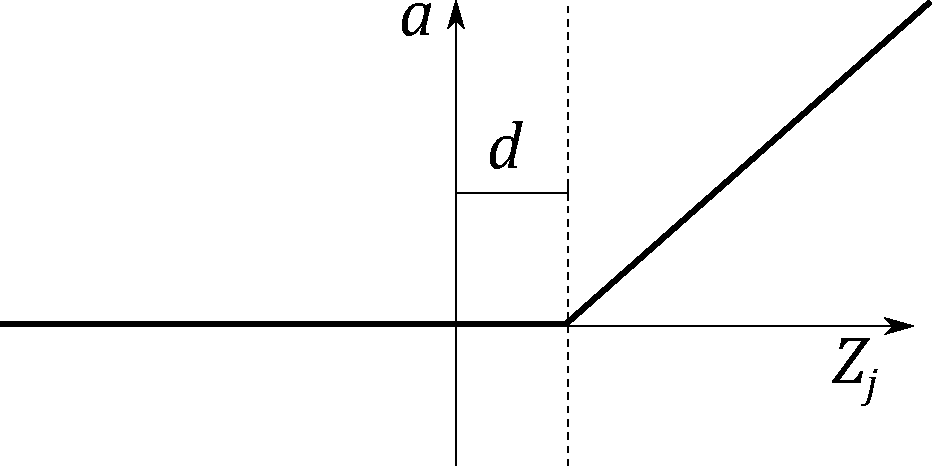
\includegraphics[width=0.5\linewidth]{images/relu.pdf}    

    \caption{In figure captions, explain what the reader is looking at: ``A schematic of the rectifying linear unit, where $a$ is the output amplitude,
    $d$ is a configurable dead-zone, and $Z_j$ is the input signal'', as well as why the reader is looking at this: 
    ``It is notable that there is no activation \emph{at all} below 0, which explains our initial results.'' 
    \textbf{Use vector image formats (.pdf) where possible}. Size figures appropriately, and do not make them over-large or too small to read.
    }

    % use the notation fig:name to cross reference a figure
    \label{fig:relu} 
\end{figure}


\begin{figure}
    \centering
    \begin{subfigure}[b]{0.45\textwidth}
        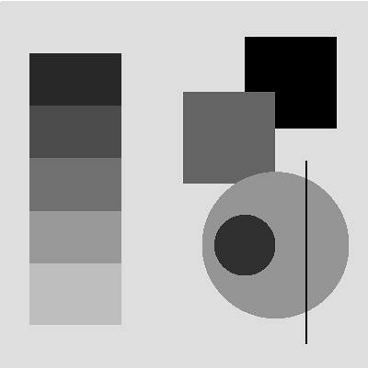
\includegraphics[width=\textwidth]{images/synthetic.png}
        \caption{Synthetic image, black on white.}
        \label{fig:syn1}
    \end{subfigure}
    ~ %add desired spacing between images, e. g. ~, \quad, \qquad, \hfill etc. 
      %(or a blank line to force the subfigure onto a new line)
    \begin{subfigure}[b]{0.45\textwidth}
        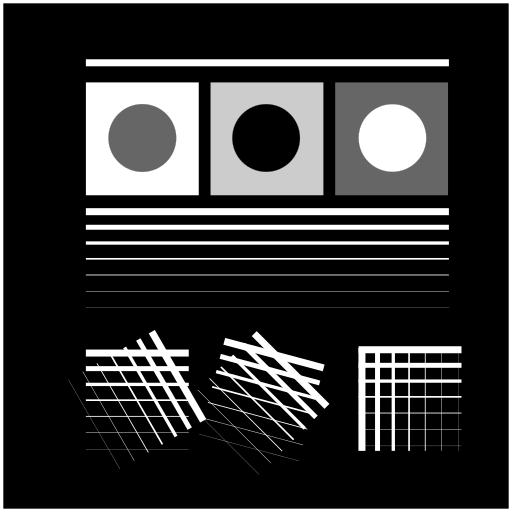
\includegraphics[width=\textwidth]{images/synthetic_2.png}
        \caption{Synthetic image, white on black.}
        \label{fig:syn2}
    \end{subfigure}
    ~ %add desired spacing between images, e. g. ~, \quad, \qquad, \hfill etc. 
    %(or a blank line to force the subfigure onto a new line)    
    \caption{Synthetic test images for edge detection algorithms. \subref{fig:syn1} shows various gray levels that require an adaptive algorithm. \subref{fig:syn2}
    shows more challenging edge detection tests that have crossing lines. Fusing these into full segments typically requires algorithms like the Hough transform.
    This is an example of using subfigures, with \texttt{subref}s in the caption.
    }\label{fig:synthetic}
\end{figure}

\clearpage

\subsection{Equations}

Equations should be typeset correctly and precisely. Make sure you get parenthesis sizing correct, and punctuate equations correctly 
(the comma is important and goes \textit{inside} the equation block). Explain any symbols used clearly if not defined earlier. 

For example, we might define:
\begin{equation}
    \hat{f}(\xi) = \frac{1}{2}\left[ \int_{-\infty}^{\infty} f(x) e^{2\pi i x \xi} \right],
\end{equation}    
where $\hat{f}(\xi)$ is the Fourier transform of the time domain signal $f(x)$.

\subsection{Algorithms}
Algorithms can be set using \texttt{algorithm2e}, as in Algorithm \ref{alg:metropolis}.

% NOTE: line ends are denoted by \; in algorithm2e
\begin{algorithm}
    \DontPrintSemicolon
    \KwData{$f_X(x)$, a probability density function returing the density at $x$.\; $\sigma$ a standard deviation specifying the spread of the proposal distribution.\;
    $x_0$, an initial starting condition.}
    \KwResult{$s=[x_1, x_2, \dots, x_n]$, $n$ samples approximately drawn from a distribution with PDF $f_X(x)$.}
    \Begin{
        $s \longleftarrow []$\;
        $p \longleftarrow f_X(x)$\;
        $i \longleftarrow 0$\;
        \While{$i < n$}
        {
            $x^\prime \longleftarrow \mathcal{N}(x, \sigma^2)$\;
            $p^\prime \longleftarrow f_X(x^\prime)$\;
            $a \longleftarrow \frac{p^\prime}{p}$\;
            $r \longleftarrow U(0,1)$\;
            \If{$r<a$}
            {
                $x \longleftarrow x^\prime$\;
                $p \longleftarrow f_X(x)$\;
                $i \longleftarrow i+1$\;
                append $x$ to $s$\;
            }
        }
    }
    
\caption{The Metropolis-Hastings MCMC algorithm for drawing samples from arbitrary probability distributions, 
specialised for normal proposal distributions $q(x^\prime|x) = \mathcal{N}(x, \sigma^2)$. The symmetry of the normal distribution means the acceptance rule takes the simplified form.}\label{alg:metropolis}
\end{algorithm}

\subsection{Tables}

If you need to include tables, like Table \ref{tab:operators}, use a tool like https://www.tablesgenerator.com/ to generate the table as it is
extremely tedious otherwise. 

\begin{table}[]
    \caption{The standard table of operators in Python, along with their functional equivalents from the \texttt{operator} package. Note that table
    captions go above the table, not below. Do not add additional rules/lines to tables. }\label{tab:operators}
    %\tt 
    \rowcolors{2}{}{gray!3}
    \begin{tabular}{@{}lll@{}}
    %\toprule
    \textbf{Operation}    & \textbf{Syntax}                & \textbf{Function}                            \\ %\midrule % optional rule for header
    Addition              & \texttt{a + b}                          & \texttt{add(a, b)}                                    \\
    Concatenation         & \texttt{seq1 + seq2}                    & \texttt{concat(seq1, seq2)}                           \\
    Containment Test      & \texttt{obj in seq}                     & \texttt{contains(seq, obj)}                           \\
    Division              & \texttt{a / b}                          & \texttt{div(a, b) }  \\
    Division              & \texttt{a / b}                          & \texttt{truediv(a, b) } \\
    Division              & \texttt{a // b}                         & \texttt{floordiv(a, b)}                               \\
    Bitwise And           & \texttt{a \& b}                         & \texttt{and\_(a, b)}                                  \\
    Bitwise Exclusive Or  & \texttt{a \textasciicircum b}           & \texttt{xor(a, b)}                                    \\
    Bitwise Inversion     & \texttt{$\sim$a}                        & \texttt{invert(a)}                                    \\
    Bitwise Or            & \texttt{a | b}                          & \texttt{or\_(a, b)}                                   \\
    Exponentiation        & \texttt{a ** b}                         & \texttt{pow(a, b)}                                    \\
    Identity              & \texttt{a is b}                         & \texttt{is\_(a, b)}                                   \\
    Identity              & \texttt{a is not b}                     & \texttt{is\_not(a, b)}                                \\
    Indexed Assignment    & \texttt{obj{[}k{]} = v}                 & \texttt{setitem(obj, k, v)}                           \\
    Indexed Deletion      & \texttt{del obj{[}k{]}}                 & \texttt{delitem(obj, k)}                              \\
    Indexing              & \texttt{obj{[}k{]}}                     & \texttt{getitem(obj, k)}                              \\
    Left Shift            & \texttt{a \textless{}\textless b}       & \texttt{lshift(a, b)}                                 \\
    Modulo                & \texttt{a \% b}                         & \texttt{mod(a, b)}                                    \\
    Multiplication        & \texttt{a * b}                          & \texttt{mul(a, b)}                                    \\
    Negation (Arithmetic) & \texttt{- a}                            & \texttt{neg(a)}                                       \\
    Negation (Logical)    & \texttt{not a}                          & \texttt{not\_(a)}                                     \\
    Positive              & \texttt{+ a}                            & \texttt{pos(a)}                                       \\
    Right Shift           & \texttt{a \textgreater{}\textgreater b} & \texttt{rshift(a, b)}                                 \\
    Sequence Repetition   & \texttt{seq * i}                        & \texttt{repeat(seq, i)}                               \\
    Slice Assignment      & \texttt{seq{[}i:j{]} = values}          & \texttt{setitem(seq, slice(i, j), values)}            \\
    Slice Deletion        & \texttt{del seq{[}i:j{]}}               & \texttt{delitem(seq, slice(i, j))}                    \\
    Slicing               & \texttt{seq{[}i:j{]}}                   & \texttt{getitem(seq, slice(i, j))}                    \\
    String Formatting     & \texttt{s \% obj}                       & \texttt{mod(s, obj)}                                  \\
    Subtraction           & \texttt{a - b}                          & \texttt{sub(a, b)}                                    \\
    Truth Test            & \texttt{obj}                            & \texttt{truth(obj)}                                   \\
    Ordering              & \texttt{a \textless b}                  & \texttt{lt(a, b)}                                     \\
    Ordering              & \texttt{a \textless{}= b}               & \texttt{le(a, b)}                                     \\
    % \bottomrule
    \end{tabular}
    \end{table}
\subsection{Code}

Avoid putting large blocks of code in the report (more than a page in one block, for example). Use syntax highlighting if possible, as in Listing \ref{lst:callahan}.

\begin{lstlisting}[language=python, float, caption={The algorithm for packing the $3\times 3$ outer-totalistic binary CA successor rule into a 
    $16\times 16\times 16\times 16$ 4 bit lookup table, running an equivalent, notionally 16-state $2\times 2$ CA.}, label=lst:callahan]
    def create_callahan_table(rule="b3s23"):
        """Generate the lookup table for the cells."""        
        s_table = np.zeros((16, 16, 16, 16), dtype=np.uint8)
        birth, survive = parse_rule(rule)

        # generate all 16 bit strings
        for iv in range(65536):
            bv = [(iv >> z) & 1 for z in range(16)]
            a, b, c, d, e, f, g, h, i, j, k, l, m, n, o, p = bv

            # compute next state of the inner 2x2
            nw = apply_rule(f, a, b, c, e, g, i, j, k)
            ne = apply_rule(g, b, c, d, f, h, j, k, l)
            sw = apply_rule(j, e, f, g, i, k, m, n, o)
            se = apply_rule(k, f, g, h, j, l, n, o, p)

            # compute the index of this 4x4
            nw_code = a | (b << 1) | (e << 2) | (f << 3)
            ne_code = c | (d << 1) | (g << 2) | (h << 3)
            sw_code = i | (j << 1) | (m << 2) | (n << 3)
            se_code = k | (l << 1) | (o << 2) | (p << 3)

            # compute the state for the 2x2
            next_code = nw | (ne << 1) | (sw << 2) | (se << 3)

            # get the 4x4 index, and write into the table
            s_table[nw_code, ne_code, sw_code, se_code] = next_code

        return s_table

\end{lstlisting}

%==================================================================================================================================
\chapter{Evaluation} 
How good is your solution? How well did you solve the general problem, and what evidence do you have to support that?

\section{Guidance}
\begin{itemize}
    \item
        Ask specific questions that address the general problem.
    \item
        Answer them with precise evidence (graphs, numbers, statistical
        analysis, qualitative analysis).
    \item
        Be fair and be scientific.
    \item
        The key thing is to show that you know how to evaluate your work, not
        that your work is the most amazing product ever.
\end{itemize}

\section{Evidence}
Make sure you present your evidence well. Use appropriate visualisations, reporting techniques and statistical analysis, as appropriate.

If you visualise, follow the basic rules, as illustrated in Figure \ref{fig:boxplot}:
\begin{itemize}
\item Label everything correctly (axis, title, units).
\item Caption thoroughly.
\item Reference in text.
\item \textbf{Include appropriate display of uncertainty (e.g. error bars, Box plot)}
\item Minimize clutter.
\end{itemize}

See the file \texttt{guide\_to\_visualising.pdf} for further information and guidance.

\begin{figure}
    \centering
    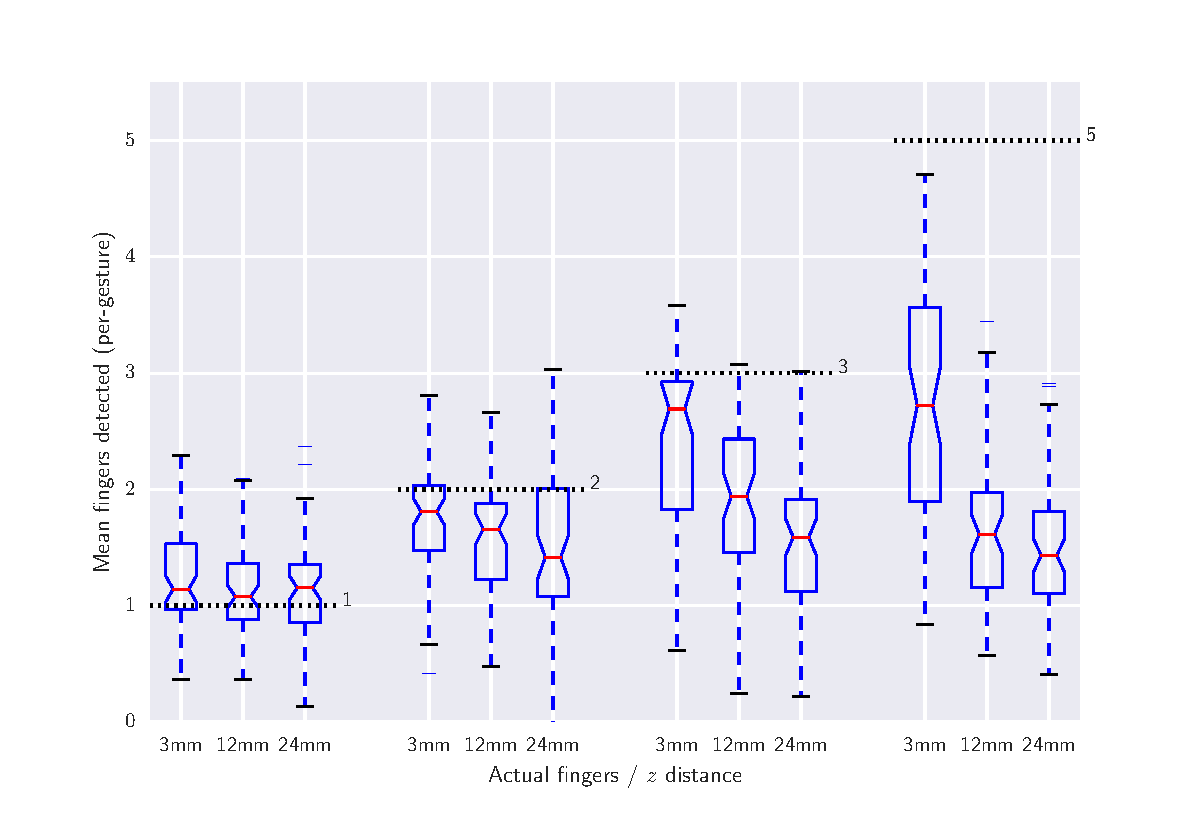
\includegraphics[width=1.0\linewidth]{images/boxplot_finger_distance.pdf}    

    \caption{Average number of fingers detected by the touch sensor at different heights above the surface, averaged over all gestures. Dashed lines indicate
    the true number of fingers present. The Box plots include bootstrapped uncertainty notches for the median. It is clear that the device is biased toward 
    undercounting fingers, particularly at higher $z$ distances.
    }

    % use the notation fig:name to cross reference a figure
    \label{fig:boxplot} 
\end{figure}


%==================================================================================================================================
\chapter{Conclusion}    
Summarise the whole project for a lazy reader who didn't read the rest (e.g. a prize-awarding committee).
\section{Guidance}
\begin{itemize}
    \item
        Summarise briefly and fairly.
    \item
        You should be addressing the general problem you introduced in the
        Introduction.        
    \item
        Include summary of concrete results (``the new compiler ran 2x
        faster'')
    \item
        Indicate what future work could be done, but remember: \textbf{you
        won't get credit for things you haven't done}.
\end{itemize}

%==================================================================================================================================
%
% 
%==================================================================================================================================
%  APPENDICES  

\begin{appendices}

\chapter{Appendices}

Typical inclusions in the appendices are:

\begin{itemize}
\item
  Copies of ethics approvals (required if obtained)
\item
  Copies of questionnaires etc. used to gather data from subjects.
\item
  Extensive tables or figures that are too bulky to fit in the main body of
  the report, particularly ones that are repetitive and summarised in the body.

\item Outline of the source code (e.g. directory structure), or other architecture documentation like class diagrams.

\item User manuals, and any guides to starting/running the software.

\end{itemize}

\textbf{Don't include your source code in the appendices}. It will be
submitted separately.

\end{appendices}

%==================================================================================================================================
%   BIBLIOGRAPHY   

% The bibliography style is abbrvnat
% The bibliography always appears last, after the appendices.

\bibliographystyle{abbrvnat}

\bibliography{l4proj}

\end{document}
